\documentclass{standalone}

\usepackage{pgfplots,tikz,amsmath}
\begin{document}
    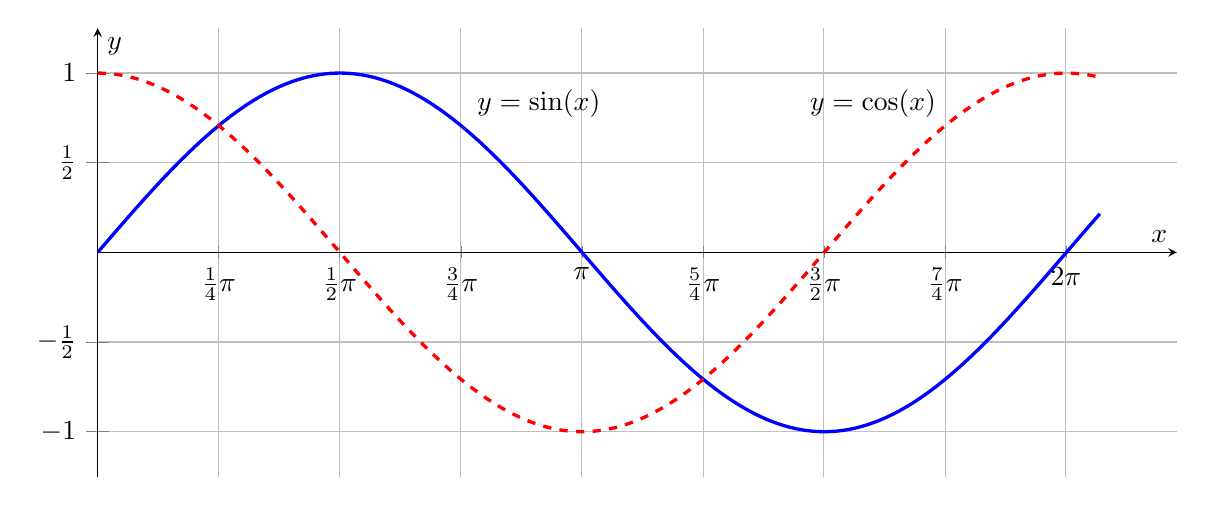
\begin{tikzpicture}
        \begin{axis}[axis lines=center, xlabel={$x$}, ylabel={$y$}, xmin=0, xmax=7,
                ymin=-1.25, ymax=1.25, ytick={-1,-0.5,0.5,1}, xtick={0.785,
                1.57, 2.356, 3.14, 3.927, 4.71, 5.498, 6.28},
                xticklabels={$\frac{1}{4}\pi$,$\frac{1}{2}\pi$, $\frac{3}{4}\pi$,$\pi$,
                $\frac{5}{4}\pi$,$\frac{3}{2}\pi$,$\frac{7}{4}\pi$,$2\pi$},
                yticklabels={$-1$,$-\frac{1}{2}$,$\frac{1}{2}$,$1$},
        grid, xscale=2]
            \addplot[smooth, very thick, color=blue, domain=0:6.5, samples=100] {sin(deg(x))};
            \addplot[smooth, dashed, very thick, color=red, domain=0:6.5, samples=100]
            {cos(deg(x))};
            \draw (axis cs:2.4,0.7) node[anchor=south west]{$y = \sin(x)$};
            \draw (axis cs:5.5,0.7) node[anchor=south east]{$y = \cos(x)$};
        \end{axis}
    \end{tikzpicture}
\end{document}
